\section{Propuesta}

\subsection{Conjunto de datos a utilizar}

Para realizar este trabajo utilizaremos un conjunto de datos con $892$ muestras de la sínfisis púbica clasificados manualmente por investigadores del Laboratorio de Antropología Física de la Universidad de Granada utilizando las diez fases propuestas por Todd.

Este conjunto de datos se divide en dos partes, las muestras tomadas de la lateralidad izquierda ($439$ muestras) y la lateralidad derecha ($453$ muestras) del pubis.

\subsubsection{Problema del balanceo de clases}

Como vimos en las figuras \ref{fig:conteo_original} y \ref{fig:conjunto_regresion} con el conteo de cada una de las fases y la densidad de las edades en el conjunto completo, los datos de este problema se encuentran altamente desbalanceados, hay rangos de edades en las que apenas contamos con datos, y la diferencia entre número de datos entre una edad temprana y alta es muy grande. De cara a resolver este problema proponemos utilizar un algoritmo de sobremuestreo de datos, al igual que \cite{NSLVOrdAge}.

En este artículo se proponen distintas técnicas de sobremuestreo, principalmente utilizando un sobremuestreo de forma aleatoria, utilizando el algoritmo SMOTE \cite{revisionSMOTE} (y varias variaciones de este algoritmo), y utilizando el algoritmo ADASYN \cite{propuestaADASYN}.

En nuestro caso, al utilizar el mismo conjunto de datos, podemos ver en su artículo que la técnica que mejor ha funcionado para este conjunto de datos es Borderline-SMOTE, sin embargo nuestro enfoque no es de clasificación, es de regresión, por lo que haremos una revisión de las adaptaciones de SMOTE a regresión y finalmente utilizaremos SMOGN, un algoritmo que utilizará un sobremuestreo con SMOTER (SMOTE para Regresión), equilibrará la densidad entre las distintas edades utilizando submuestreo en caso de que no pueda generar nuevos datos sintéticos y añadirá ruido gaussiano de cara a adaptar los nuevos datos a un problema de regresión.

\subsubsection{Enfoque con el que trabajaremos el conjunto de datos}

De cara a resolver el problema y obtener un buen estimador de la edad a partir de los huesos del pubis enfocaremos el problema como un problema de regresión. Utilizaremos la propuesta de Gilbert y McKern para transformar las características a valores numéricos, que serán la entrada del modelo que entrenemos.

El modelo devolverá como resultado la expresión que mejor se ajuste a los datos con los que se ha entrenado el modelo, y será esa expresión con la que validaremos el modelo.

\begin{figure}[H]
    \centering
	  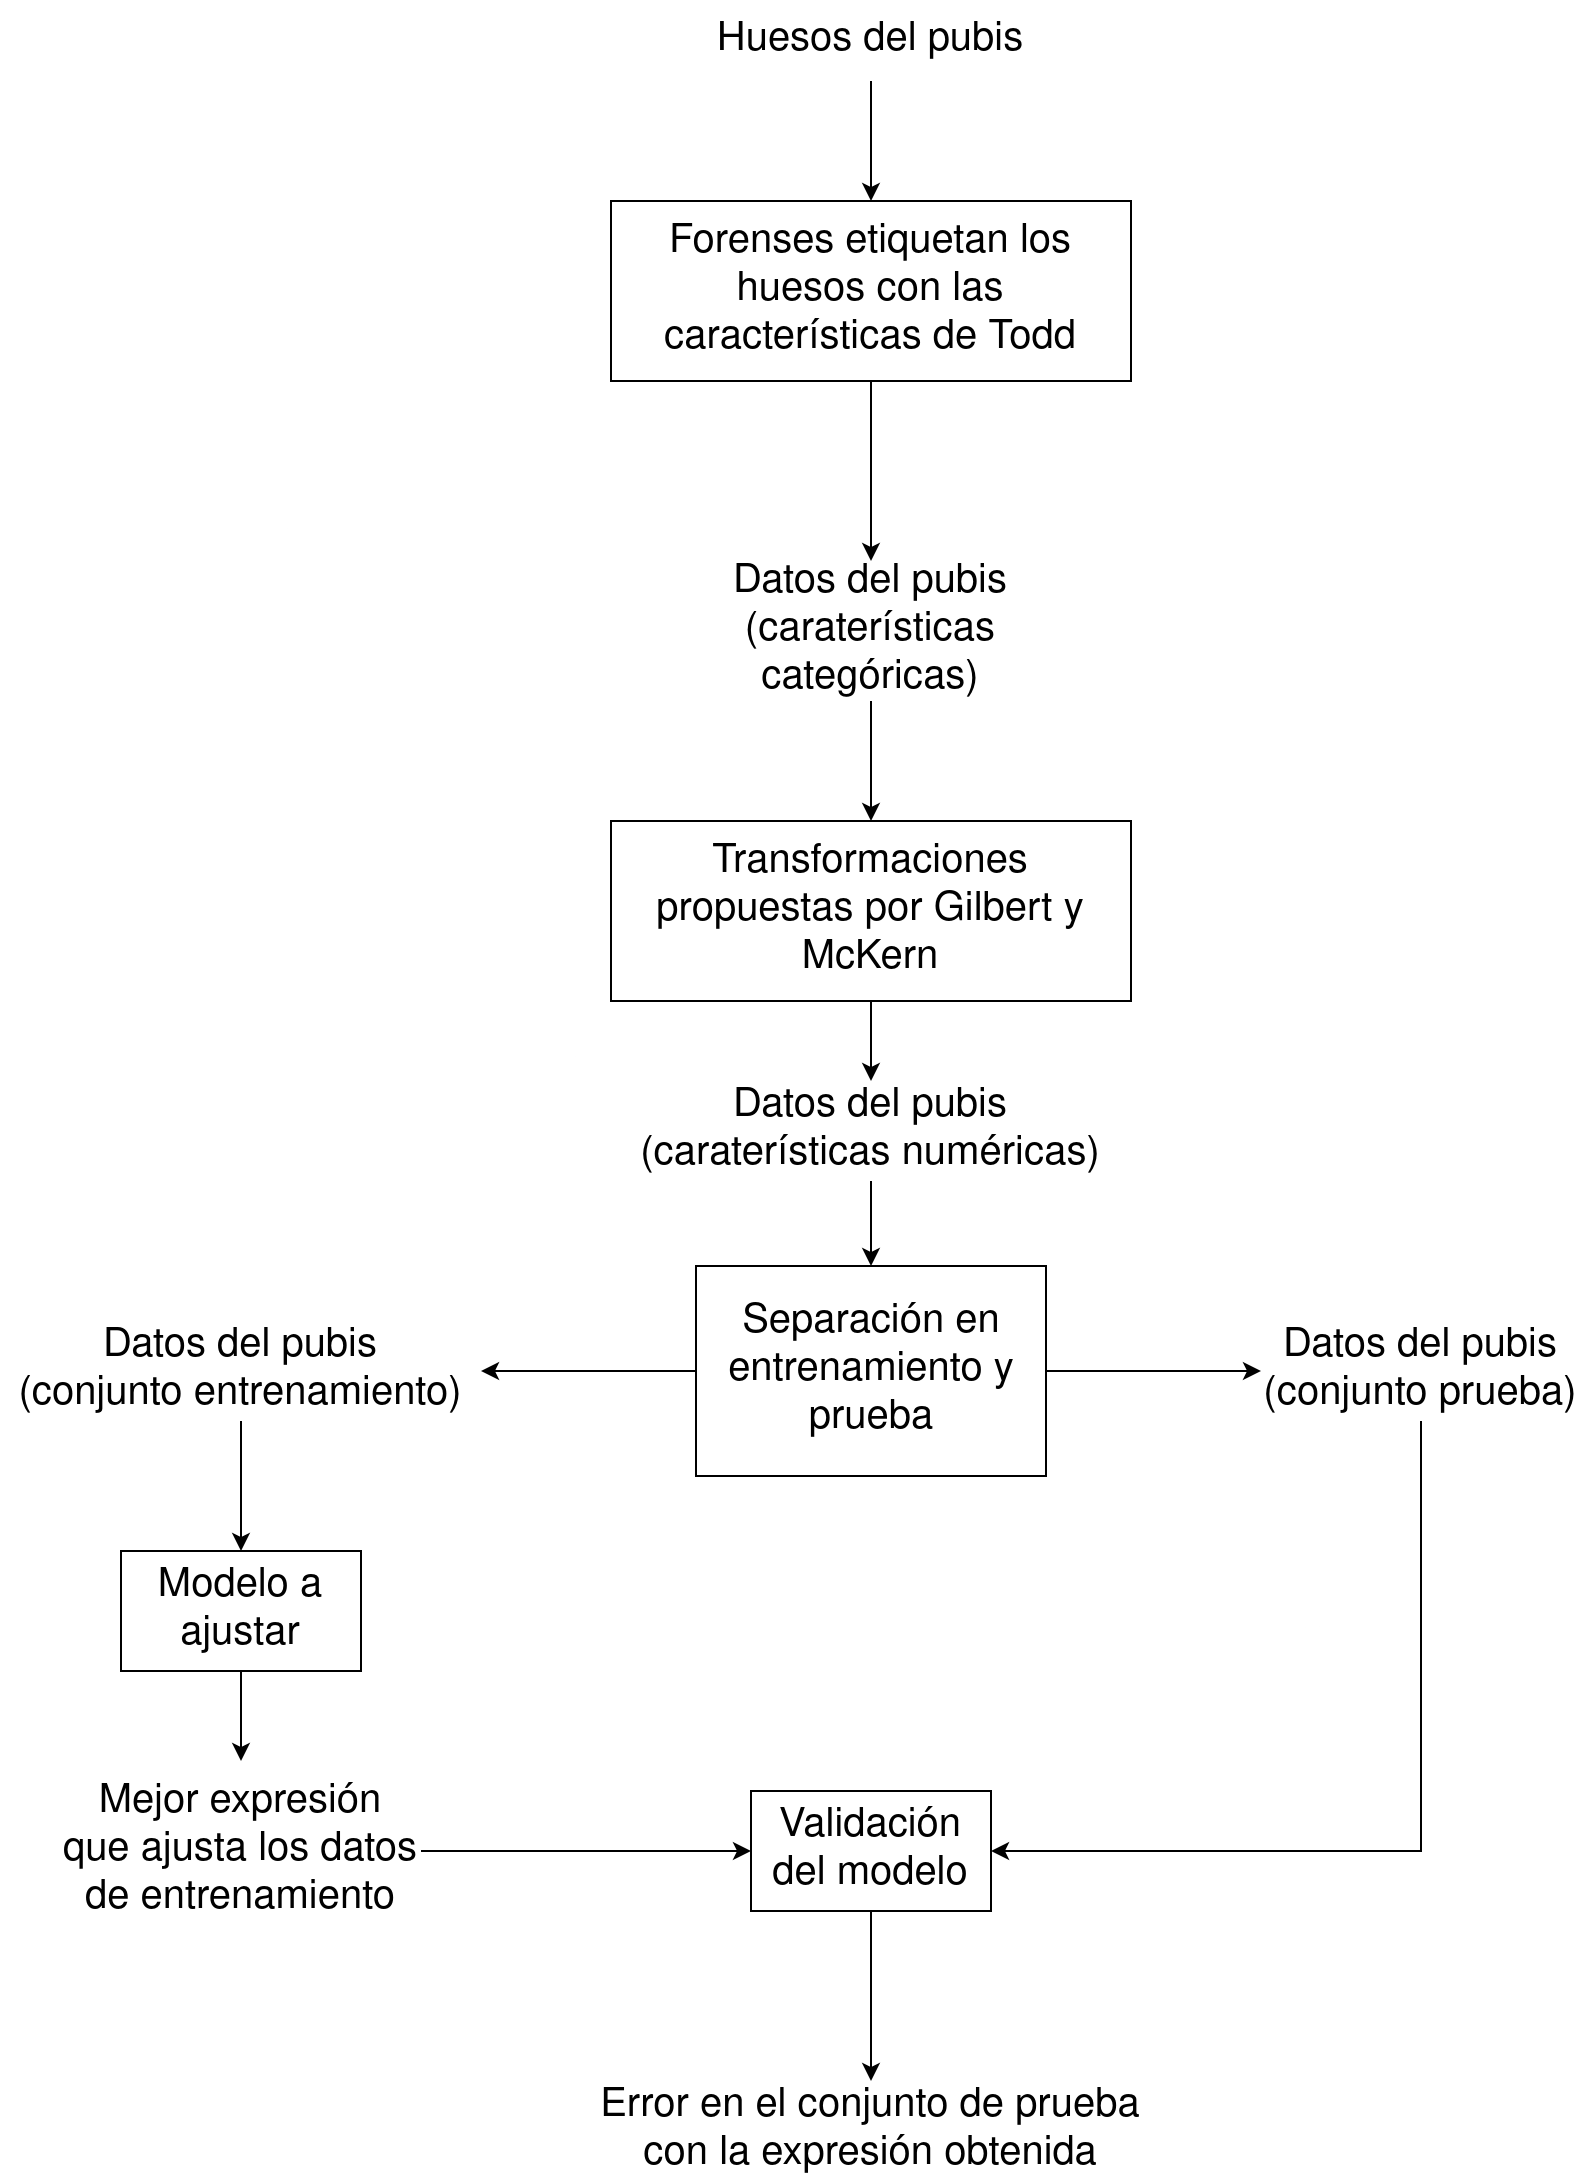
\includegraphics[width=0.8\textwidth]{esquema_datos.png}
    \caption{Esquema general de los pasos que seguirá el conjunto de datos para entrenar y validar el modelo.}
	 \label{fig:esquema_datos}
\end{figure}

En la figura \ref{fig:esquema_datos} podemos ver el flujo que seguirán los datos de entrada, a falta de concretar el sistema de validación a utilizar, 5x2cv, que se explicará más adelante.

\newpage

\subsection{Algoritmos a utilizar e implementación}

Para resolver este problema utilizaremos el algoritmo de Programación Genética y su variante GA-P. Hemos escogido estos algoritmos ya que se tratan de algoritmos cuyas soluciones son sencillas de entender y además, como hemos visto en el estado del arte y antecedentes, estos algoritmos funcionan muy bien para regresión simbólica, con la que le podemos dar un nuevo enfoque al problema.

De cara a la implementación se propone utilizar \textit{Python} para aplicar parte del preprocesado de los datos ya que este lenguaje cuenta con múltiples herramientas para análisis de datos, mientras que para la implementación de los algoritmos se utilizará \textit{C++}.

La decisión de utilizar \textit{C++} viene dada ya que estos algoritmos tienden a ser lentos a la hora de realizar su entrenamiento, por lo que se ha buscado un lenguaje compilado con el que tener mejores tiempos de ejecución. También nos permite realizar una implementación orientada a objetos, lo que nos dará una mejor estructura del código a implementar, así como utilizar software como \textit{OpenMP} \cite{OpenMP} de cara a paralelizar secciones de código que nos permiten reducir el tiempo de ejecución gracias al paralelismo de datos, como veremos más adelante.

Por último, este lenguaje nos ofrece distintas herramientas de control del software, como \textit{GDB} \cite{gdb} para depurar el código, \textit{Valgrind} \cite{valgrind} para comprobar que no existen problemas con la memoria dinámica y la biblioteca \textit{Google Test} \cite{gtest} para realizar test unitarios y comprobar que el código funciona correctamente.

También se utilizará el sistema de control de versiones \textit{Git} \cite{git} durante todo el proceso de creación del código y esta memoria.

% \subsection{Planificación temporal}

\newpage
